%!TEX TS-program = xelatex
%!TEX root = ../../maxwell2018thesis.tex

\chapter[Information Retrieval]{Information Retrieval:\\A History and Background}\label{chap:ir_background}
It may be fair to say that \emph{searching for information} is now a commonplace activity within our daily lives. Given the familiarity and near ubiquity of the search box (as shown below) on contemporary human-computer interfaces, one may be forgiven into na\"{i}vely thinking that research and development into the underlying \emph{search engine} that one interacts with when using the search box was focused exclusively upon the domain of \emph{web search}, where names like \emph{Google}, \emph{Bing} and \emph{AltaVista}\footnote{This name might spring to mind for those with more of a historical knowledge of search engines. The author of this thesis has very vague memories using AltaVista when he was around eight years old\dots} spring to mind. Despite potential negatives that these technologies may bring -- turning us into so-called \emph{shallow thinkers}~\citep{carr2008google_stupid}, for example -- search engines today by and large make our lives easier, allowing us to find that proverbial needle in the haystack with relative ease.

\begin{figure}[h]
    \centering
    \vspace{4mm}
    \resizebox{1\hsize}{!}{
    
\includegraphics{figures/ch2-searchbox.pdf}}
    \label{fig:searchbox}
    \vspace{-5mm}
\end{figure}

The research and development that has gone into search and indexing technologies that allow us to find that proverbial needle has been going on for decades, long before the advent of computers and associated communication technologies, such as the~\gls{acr:www}. This research has led to the formation of the study of~\gls{acr:ir} and the development of contemporary~\gls{acr:ir} systems.\footnote{Some within the~\gls{acr:ir} may consider this to be a contentious point: does the~\gls{acr:ir} community embrace those wishing to contribute? One of the most famous research papers associated with~\gls{acr:ir} discussing Google's \emph{PageRank} algorithm~\citep{page1998pagerank}, was rejected from SIGIR. See \url{http://rakaposhi.eas.asu.edu/f08-cse494-mailarchive/msg00037.html} (last accessed March 6\textsuperscript{th}, 2018) for more information.} With this field of study has come with it the development a \emph{de facto} approach to conducting~\gls{acr:ir} research, along with various retrieval models and means with which to evaluate their effectiveness. It is in this vain that we frame this chapter: beginning with a brief history of~\gls{acr:ir} research (Section~\ref{sec:ir_background:history}), we then consider the basic assumptions and approaches used within the field for experimental research (Section~\ref{sec:ir_background:basics}) and how we evaluate these experiments (Section~\ref{sec:ir_background:evaluation}).

\section{A (Brief) History of Information Retrieval}\label{sec:ir_background:history}
It has only been over the last two decades that search engines have become commonplace in our daily lives, primarily for the domain of web search -- as discussed in Section~\ref{sec:ir_background:history:www}. Contemporary search technologies are essentially ubiquitous, integrating seamlessly with computer operating systems (as illustrated in Figure~\ref{fig:search_integration}). Computerised~\gls{acr:ir} systems have however existed as far back as the late 1940's (as demonstrated by~\citealp{holmstrom1948univac}), with more primitive approaches (both mechanised and manual categorisation approaches) to sorting and categorising information being developed even earlier.

\begin{figure}[t!]
    \centering
    \resizebox{1\hsize}{!}{
    
\includegraphics{figures/ch2-search_integration.png}}
    \caption[Search Integration within Windows\textregistered~10]{An example of search integration within the Windows\textregistered~10 operating system. Here, results for the query \texttt{glasgow university} are shown. Results are returned from the \emph{Bing} search engine; one can also search for files on their local computer.}
    \label{fig:search_integration}
\end{figure}

\subsection{Libraries and Mechanisation}
Before the advent of computers and technologies such as the~\gls{acr:www}, one of the first locations in which one would consult when looking for information would be a \emph{library}. Containing a large volume of books discussing a virtually unlimited range of categories, the need for providing a means to organise (and thus locate) information with relative ease was of paramount importance. \emph{Catalogues} provide such a way in which to do this, with ancient Greek poet Callimachus being the first person to create such an item, in the third century BC~\citep{eliot2009companion}. A more recognisable approach to categorising content was devised by~\cite{dewey1891dcs} with the \emph{Dewey Decimal System}. The use of cards as an \emph{indexing system} was also considered by individuals such as~\cite{soper1920patent} who invented a system of providing information on what category a card belonged to based upon a punched hole.

In order to speed up the process of finding useful material, mechanisation was also extensively used. Allowing for searching at the rate of 600 cards per minute, Luhn devised in the early 1950's a mechanised system which utilised punchcards and light. As stated by~\cite{sanderson2012history_of_ir}, this was also around the time that the term~\glsfirst{acr:ir} was used~\citep{mooers1950theory}. It was at this point that computer technology was rapidly developing as a base for a viable, faster alternative to manual and mechanised approaches. This therefore led to the demise of mechanised systems, as highlighted by~\cite{jahoda1961electronic_searching}.

\subsection{The Rise of Computers}
Computers today provide the medium with which we closely associate a typical~\gls{acr:ir} system.~\cite{sanderson2012history_of_ir} state that digital storage capacity (e.g. hard disks) roughly doubles every two years -- similar to the famous \emph{Moore's Law}~\citep{moore1965law}, which observes that the number of transistors in a processor (or integrated circuit) doubles roughly every two years. Indeed, the speed at which contemporary computers can search vast indexes and databases of content is vastly superior to traditional cataloguing approaches.

One of the earliest discussions about the use of computers as the basis for an~\gls{acr:ir} system specifically mentioned the~\gls{acr:univac}.~\cite{holmstrom1948univac} described a (potentially pre-production)~\gls{acr:univac} system that was capable of searching for text with a given \emph{reference code} stored on steel tape.~\cite{mitchell1953univac_million} also showed a~\gls{acr:univac} system capable of searching one million records indexed by six subject codes. It was around this time that computers began to replace the traditional librarian, being able to provide a much more effective and cost effective means of trawling through a library's records.

From this point on, work began to establish~\gls{acr:ir} as a scientific field. Gerard Salton established a large~\gls{acr:ir} research group, initially at Harvard University. Many of the basic constructs which we utilise within~\gls{acr:ir} today were established around this time, in addition to the experiments undertaken by~\cite{cleverdon1962cranfield_experiments} -- known as the \emph{Cranfield Experiments}. These experiments established the concept of using words to index documents within an~\gls{acr:ir} system, providing advancements in indexing technology.~\cite{luhn1957ranking_query} proposed, and~\cite{maron1959probabilistic_indexing} tested, an approach to ranking that scored documents in a collection in relation to a user issued \emph{query} -- a concept that is central to contemporary~\gls{acr:ir} systems. A detailed explanation of these concepts are provided later in this chapter -- refer to Section~\ref{sec:ir_background:basics}.

\begin{figure}[t!]
    \centering
    \resizebox{1\hsize}{!}{
    
\includegraphics{figures/ch2-yahoo.png}}
    \caption[Screenshot of \emph{Yahoo!} Search, July 1998]{A screenshot of the landing page of \emph{Yahoo!}, as shown on July 5\textsuperscript{th}, 1998. Notice the link for the 1998 \emph{FIFA World Cup} that was taking place at the time the page was created. More central to this thesis is the inclusion of a list of page categories in conjunction with the now ubiquitous search box. Screenshot acquired from the \href{https://web.archive.org/web/19980705003104/http://www.yahoo.com}{\emph{Internet Archive}}.}
    \label{fig:yahoo}
\end{figure}


\subsection{The World Wide Web}\label{sec:ir_background:history:www}
The distribution and ability to search for information over computer networks such as the internet was traditionally undertaken with legacy protocols such as \emph{Gopher}. Gopher would provide a series of options for a user to select (i.e. categorisation), akin to the traditional library cataloguing approaches described above.

The advent of the~\gls{acr:www} in the early 1990's brought about a new type of search engine -- \emph{web search engines}. Regarded as the first experimental web search engine, \emph{JumpStation} was described by~\cite{mcbryan1994taming_tools}. In this system, \emph{anchor text} within \emph{hyperlinks} of~\gls{acr:html} pages could be exploited to aid the ranking of documents. However, popular search engines of the 1990's initially followed the categorisation approach hailing back from libraries, as illustrated in Figure~\ref{fig:yahoo} with a screenshot of \emph{Yahoo!} from 1998. However, as the volume of information on the~\gls{acr:www} began to increase, this approach became impractical. As such, it was not long before a more contemporary search engine took ahold, with the search box, allowing searchers to pose their own \emph{queries}, becoming the dominant (and defining) symbol of search. Algorithms such as Google's PageRank~\citep{page1998pagerank} took hold, with this algorithm credited for cementing Google's dominance of the search market. Over the past two decades, there have been many advances from these initial approaches to developing~\gls{acr:ir} systems. For example, the exploitation of interaction logs have become commonplace in search engines to assist in providing higher quality results, and a more personable experience for searchers.

\section{Information Retrieval Basics}\label{sec:ir_background:basics}
As may have already been surmised, the key purpose of an~\gls{acr:ir} system is to locate information that is relevant to a searchers's information need. Such a system would search through collection(s) of \emph{unstructured} or \emph{semi-structured} data (such as a collection of web pages, documents, images, videos, etc.), before returning potential matches to the searcher. 

\blueboxheader{Unstructured vs. (Semi-)Structured Data}
The examination of unstructured or semi-structured data is a key difference of an~\gls{acr:ir} system when compared to a~\gls{acr:rdbms}, for example (see Figure~\ref{fig:structured_data}). With a~\gls{acr:rdbms}, data is inherently structured based upon some predetermined \emph{schema}. With an~\gls{acr:ir} system, such a premise for structured data does not exist.\footnote{This may be a slight misnomer; schemas can be used for an~\gls{acr:ir} system index when considering \emph{fielded retrieval}. For example, a collection of newspaper articles may contain a title and body -- but within the fields, the data is unstructured.} Semi-structured data such as an~\gls{acr:html} page contains a series of \emph{elements} (e.g. \texttt{<h1>} for headers), but the text within these tags is largely of an unstructured nature. The unstructured data can contain information such as dates or entities (terms describing a real-world object and/or location, such as \texttt{canberra} or \texttt{dropbear}, and can be -- as it is probably written in a natural language -- ambiguous. As such, unstructured data presents a major challenge to address, and is the cornerstone of~\gls{acr:ir} research.

\begin{figure}[t!]
    \centering
    \resizebox{1\hsize}{!}{
    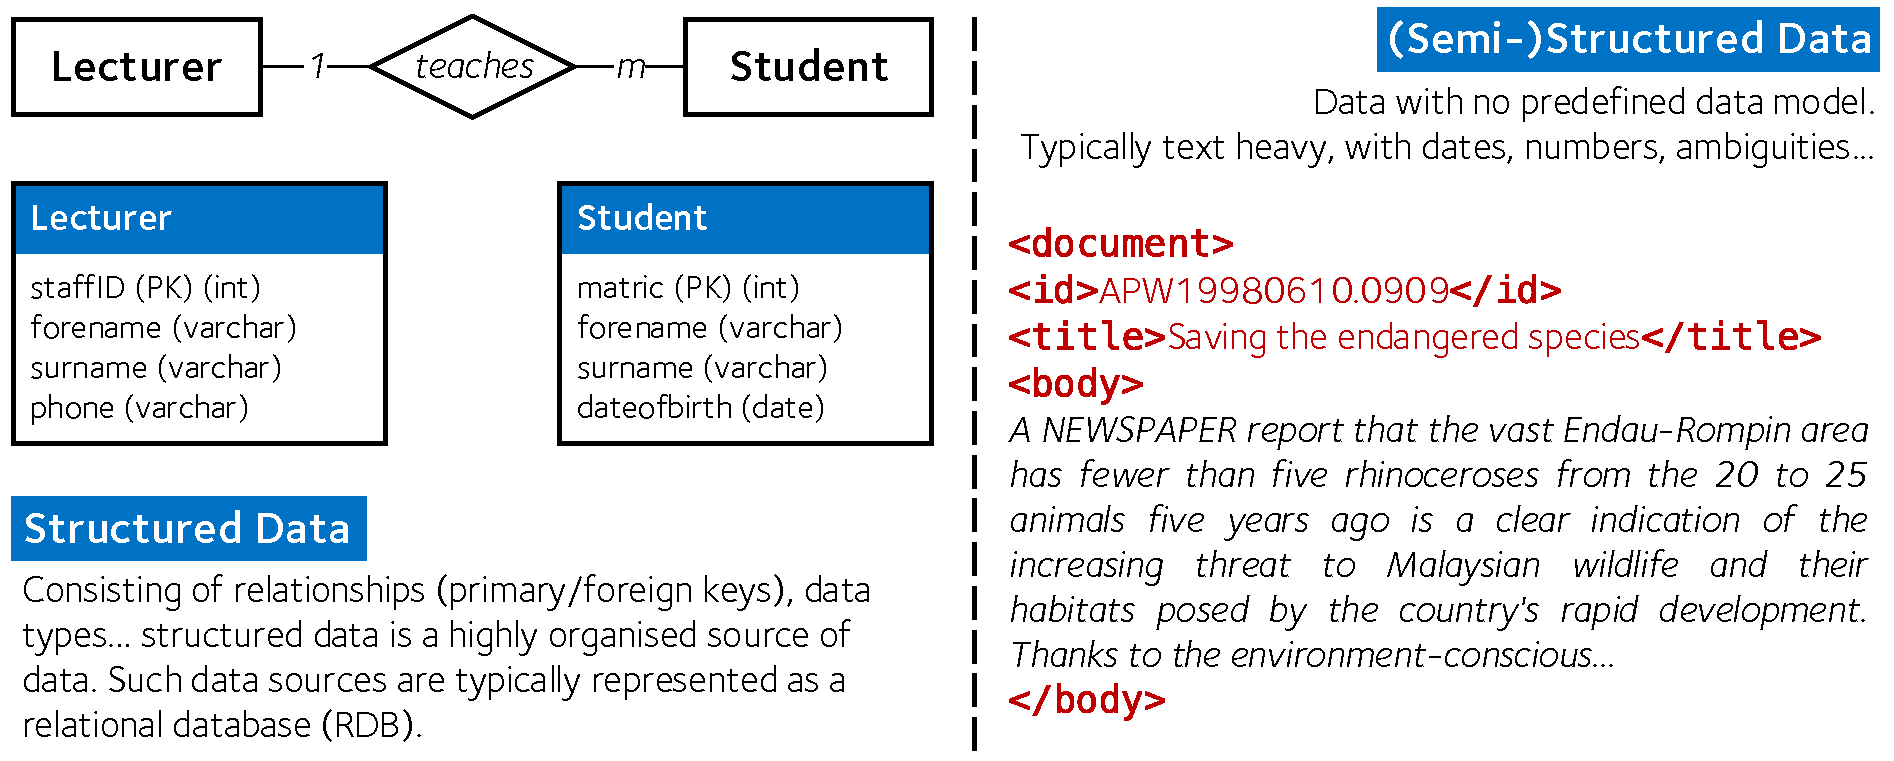
\includegraphics{figures/ch2-structured.pdf}}
    \caption[Structured and (semi-)structured data]{Examples of structured and (semi-)structured data. On the left is a structured~\gls{acr:rdbms} schema, represented in compressed Chen notation. Different types can be specified for each field, representing data in a structured way. On the right, semi-structured data, using a document from the \emph{TREC AQUAINT} newswire collection. Note the semi-structured component at the top of the document (containing an identifier and title), and the unstructured body text.}
    \label{fig:structured_data}
\end{figure}

To complement this challenge, a contemporary~\gls{acr:ir} system is also expected by its users to return results that can be considered \emph{useful} to addressing the searcher's information need, as hypothesised by~\cite{luhn1957ranking_query}, and succinctly expressed by~\cite{robertson1977prp}.

\begin{quote}
    ``A [reference] retrieval system should rank references in the collection in order of their probability of relevance to the request, or of usefulness to the user, or of satisfying the user.''
    \attrib{\cite{robertson1977prp}}
\end{quote}

\blueboxheader{Queries and Results}
A searcher's information need is represented as a \emph{query}. which is in turn comprised of one or more salient \emph{query terms}. The process of converting an information need to a query is known as \emph{query formulation}~\citep{hiemstra2009ir_models}. Depending upon the search domain, the query language used may be artificial. For example, reserved keywords may be utilised to express a \emph{boolean query} (e.g. use of \texttt{AND} or \texttt{NOT} preceding terms -- refer to Section~\ref{sec:ir_background:basics:models:boolean} for more information). Natural language however is considered to be the preferred choice within an~\gls{acr:ir} context~\citep{rijsbergen1979ir}. Given the claim by~\cite{robertson1977prp} above, an~\gls{acr:ir} system then typically returns a series of documents. Depending upon the type of system used, these results my be ranked in order of decreasing perceived relevance by some form of \emph{retrieval model}. The presentation of these results are perhaps known best as the \emph{ten blue links}~\citep{hearst2009_search}, a name given to the way in which web search engines traditionally present results to searchers. If none of the results returned to the searcher can be considered useful in any way to addressing his or her information need, the underlying~\gls{acr:ir} system is largely considered to have failed the searcher~\citep{rijsbergen1979ir}.

\blueboxheader{Operational and Experimental Systems}
\cite{rijsbergen1979ir} defines a difference between \emph{operational} and \emph{experimental}~\gls{acr:ir} systems. While a majority of individuals will only ever interact with an operational, probably commercial~\gls{acr:ir} system (e.g. Google), the work described in this thesis considers purely experimental systems. In order for one to determine how well a particular experimental~\gls{acr:ir} system performs compared to others, a rigid scientific methodology must be employed to allow for fair comparisons. As such, the remainder of this chapter discusses the \emph{de facto} approach that is considered for~\gls{acr:ir} experimentation -- from the setup of such an~\gls{acr:ir} system to the ways in which they can be evaluated.

\subsection{The Cranfield Model}\label{sec:ir_background:basics:cranfield}
The methodology behind the majority of contemporary~\gls{acr:ir} research has centred around the concept of the so-called \emph{Cranfield Model}. Devised, unsurprisingly, at Cranfield University in Bedfordshire, England, the model is based upon the \emph{Cranfield II} experiments~\citep{aslib1966factors}. As highlighted by~\cite{borlund2003iir_model}, the experiments revolve around the notion of \emph{test collections}, with the basic components of the experimental setup illustrated in Figure~\ref{fig:ir_cranfield}. Essentially, the concept of test collections is comprised of three main components.

\begin{itemize}
    \item{A collection of \emph{documents} is provided, which is typically converted to an inverted index before experimentation can begin (refer to Section~\ref{sec:ir_background:basics:indexing}).}
    \item{A collection of \emph{topics} provide a means of simulating different information needs -- and with each topic are one or more \emph{queries} that can be issued to an experimental~\gls{acr:ir} system.}
    \item{Finally, a collection of \emph{relevance assessments} are provided as part of the collection.}
\end{itemize}

\begin{figure}[t!]
    \centering
    \resizebox{1\hsize}{!}{
    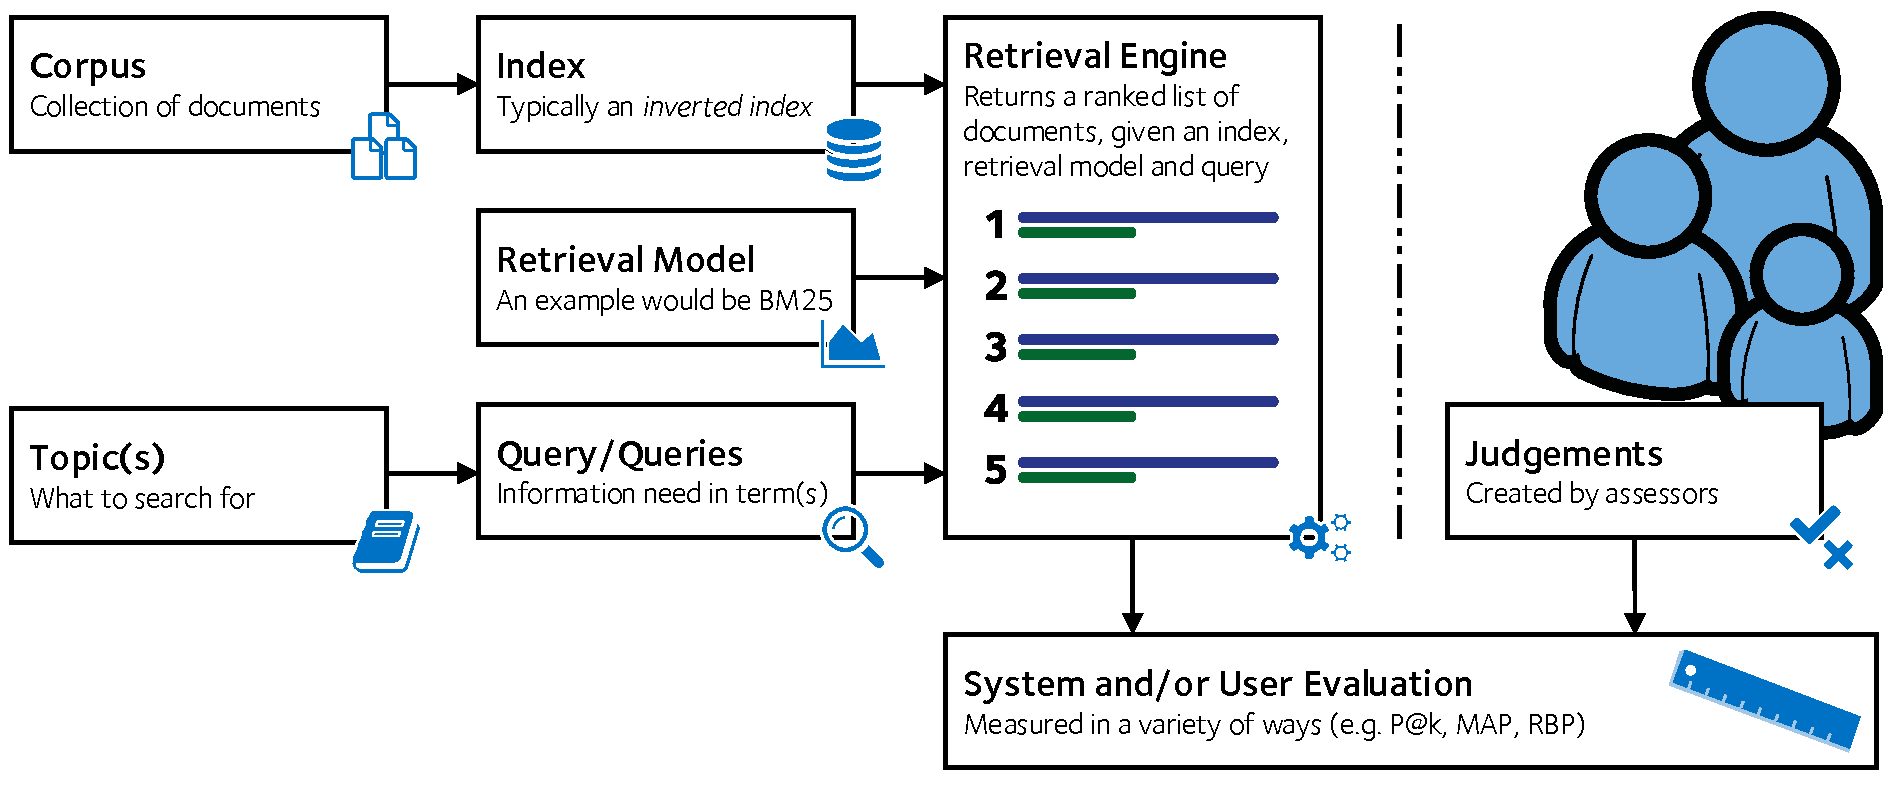
\includegraphics{figures/ch2-cranfield.pdf}}
    \caption[The \emph{Cranfield Model}]{Illustration of the Cranfield Model, the \emph{de facto} approach experimental methodology used for~\gls{acr:ir} research. Given a corpus, topic(s) and document judgements (created by assessors), one can compute various evaluation measures for a given retrieval model and search engine.}
    \label{fig:ir_cranfield}
\end{figure}

In conjunction with the documents and topics, a \emph{retrieval model} is employed (refer to Section~\ref{sec:ir_background:basics:models}), which encapsulates our beliefs about the nature of what constitutes \emph{useful} content. When instantiated, these components are in turn used by the \emph{retrieval engine} to produce a list of potentially useful documents -- called the \emph{matching process}. Many experimental retrieval engines exist, with a non-exhaustive list including: the \emph{Terrier~\gls{acr:ir} platform}\footnote{\url{http://terrier.org/}}; \emph{Apache Lucene}\footnote{\url{https://lucene.apache.org/}}; and \emph{Whoosh}\footnote{\url{https://pypi.python.org/pypi/Whoosh/} -- all URLs mentioned in this footnote were last accessed on March 8\textsuperscript{th}, 2018. \todo{Check they are all on the same page.}}. A specific retrieval engine can be selected based upon the requirements and existing infrastructure available for the particular experiment. In this thesis, for example, we rely upon the Whoosh retrieval engine for all experimental work. Output from the experimental system can then be evaluated using an \emph{evaluation tool} to produce a series of measures to examine the performance of the system (refer to Section~\ref{sec:ir_background:evaluation}).

Relevance assessments are created for each topic of the collection. Assessors examine a series of documents that are extracted from the document collection using a simple query (called \emph{pooling}). For example, given a topic \texttt{wildlife extinction}, a query typically issued to retrieve documents will also be \texttt{wildlife extinction}. The returned documents are then assessed for relevance to the given topic, and a judgement is assigned to each. Typically, such a judgement has been binary, with \texttt{0} denoting non-relevant, and \texttt{1} denoting relevant. The effects of pooling can mean that documents that are potentially relevant can be missed by assessors, and thus will receive no judgement~\citep{keenan2001effect}.

\subsubsection{The Text REtrieval Conference}\label{sec:ir_background:basics:cranfield:trec}
A number of different evaluation forums have been borne out of the Cranfield model. Perhaps most notably is~\gls{acr:trec}, as sponsored by the U.S. Government funded \emph{National Institute for Standards and Technology (NIST)}. Other efforts which have been inspired by~\gls{acr:trec} include \emph{NTCIR}, \emph{CLEF} and \emph{INEX}. Experimentation following the original~\gls{acr:trec} approach is named\emph{~\gls{acr:trec}-style} in this thesis.

Originally organised by Donna Harman and Ellen Voorhees,~\gls{acr:trec} provides a platform for annual collaboration between research groups interested in different aspects of~\gls{acr:ir} research. Each year, a series of~\gls{acr:trec} \emph{tracks} are defined, with each consisting of a collection of documents, topics and relevance judgements. Those who provide the judgements are assessors, usually employees of NIST~\citep{robertson2008history_ir_evaluation}, who were in turn previously employed as news analysts by various U.S. security agencies. Each team wishing to participate in a track receives the collection, and runs them through their experimental search system, following the approach illustrated in Figure~\ref{fig:ir_cranfield}.

Output from the experiments should then be produced in a standardised format. Results can then be used in conjunction with the judgements (termed \emph{Query RELevance judgements}, or \emph{QRELs}), again, as illustrated in Figure~\ref{fig:ir_cranfield}, and fed into a standardised program called \texttt{trec\_eval}\footnote{\texttt{trec\_eval} is downloadable from \url{http://trec.nist.gov/trec_eval/} -- URL last accessed on March 8\textsuperscript{th}, 2018. Version 8.1 of the software was used for computing most of the evaluation measures reported in this thesis.} to perform evaluation of the runs that are undertaken. The application returns the values for a number of common system-sided evaluation measures, some of which are discussed in Section~\ref{sec:ir_background:evaluation}. 

The collaborative (and perhaps competitive) atmosphere that TREC has fostered has broadly been accepted to be good for the~\gls{acr:ir} community. As discussed by~\cite{robertson2008history_ir_evaluation}, some of the main advantages of~\gls{acr:trec} is that it has encouraged a good, formalised scientific methodology for~\gls{acr:ir}. In addition, the provision of providing the community with a large volume of standardised test materials of the quality and quantity in which~\gls{acr:trec} has done is nothing like what was previously available.~\cite{robertson2008history_ir_evaluation} goes on to claim that simply examining the number of research papers published in the field employing some form of~\gls{acr:trec} data is substantial, and that alone is enough to justify the existence of the forum. Standardised sets should also aid reproducibility of research, although we acknowledge that there are other factors at play in order to achieve that goal. 

As previously mentioned,~\gls{acr:trec} is comprised of a series of different tracks, each with its own set of tasks. Some of the tasks, such as those in the \emph{Interactive Track}, as what as known as \emph{ad-hoc}. This type of task can be considered as one of the most obvious for search, when a searcher develops a need for information, and then issues a query to an underlying search engine. Tasks like ad-hoc essentially provide a form of \emph{user model}, one that has been extensively used within~\gls{acr:ir} research for a number of decades. Section~\ref{sec:ir_background:user:trec} provides more information on the steps involved in the model, and what it assumes.

\subsection{Indexing Documents}\label{sec:ir_background:basics:indexing}
As previously discussed, the conversion of a series of documents (corpus) into a data structure facilitating fast, full-text search -- as required of an~\gls{acr:ir} system -- is known as \emph{indexing}. This full-text searching is undertaken, usually in milliseconds, in aid of finding useful documents for a given query. Without an index, a retrieval engine would have to manually examine each and every document within a corpus. This would require significant computational power -- and is indeed infeasible for a large scale index, such as the index used in a contemporary commercial web search engine. The additional storage space and management required to maintain an index of documents is considered to be a necessary tradeoff to guarantee timely responses to queries.

\begin{figure}[t!]
    \centering
    \resizebox{1\hsize}{!}{
    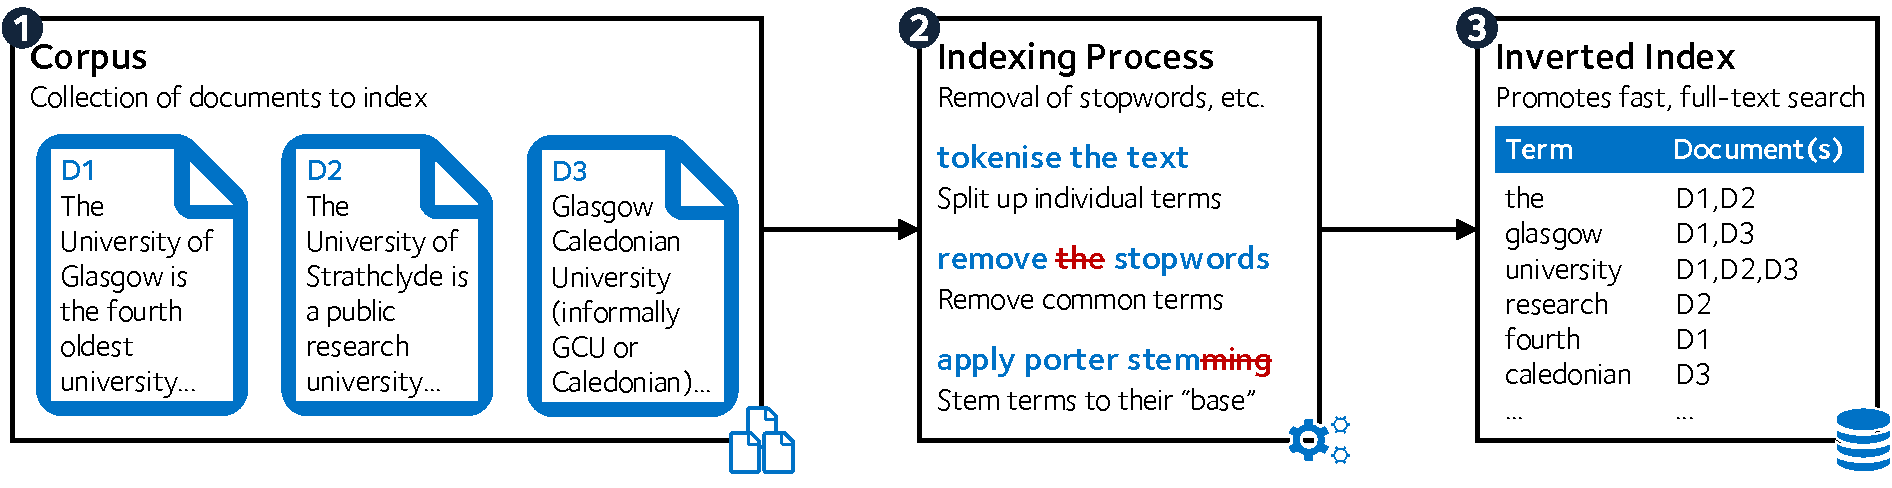
\includegraphics{figures/ch2-inverted.pdf}}
    \caption[Illustration of an \emph{Inverted index}]{A demonstration of an \emph{inverted index}, with three source documents for comparison. Depending upon the requirements of the~\gls{acr:ir} system, the indexing process may vary; all classical~\gls{acr:ir} systems however rely upon some form of inverted index.}
    \label{fig:inverted}
\end{figure}

As illustrated in Figure~\ref{fig:inverted}, the indexing process can be split into three main steps: 

\begin{itemize}
    \item{gathering the corpus of documents to be indexed;}
    \item{performing pre-indexing data preparation; and}
    \item{creating the inverted index.}
\end{itemize}

For the purposes of IR experimentation, most corpora are provided in from the evaluation forum providing the raw materials. As an example, at the time of writing, the University of Glasgow provides the TREC \emph{W2Tg}, \emph{WT10g}, \emph{.GOV} and \emph{.GOV2} document collections.\footnote{Refer to \url{http://ir.dcs.gla.ac.uk/test_collections/} -- URL last accessed March 10\textsuperscript{th}, 2018.}

Running~\gls{acr:ir} experiments with provided test collections is the case for~\gls{acr:ir} experiments following the Cranfield model -- including, of course, TREC experimentation (refer to Section~\ref{sec:ir_background:basics:cranfield:trec}), and the work presented in this thesis. For operational~\gls{acr:ir} systems, data is collated by other means. For example, web search engines employ a \emph{crawler} to examine pages on the~\gls{acr:www} and accumulates more content by following the web's hyperlink structure. Google's crawler for example is called the \emph{Googlebot}, and regularly crawls high impact websites (e.g. popular news sites, such as \emph{BBC News}) to ensure that the associated index is continually refreshed with up to date information. The enormous size of an index that would be employed by Google for web search -- as well as the need for it to be continually updated -- is itself a major engineering challenge, and is not covered in this chapter.

With the indexing process examining each document within the corpora under consideration, a complete \emph{index} will contain an entry for each processed document along with a \emph{vector} of terms that are present within said document. This is known as the \emph{forward index}. An~\gls{acr:ir} system however needs to support fast full-text search, matching terms from a searcher's query to one or more documents within the corpora. To support faster query matching, the most simplistic approach is to \emph{invert} the index, such that the lookup of the index then corresponds to an individual term. A vector of \emph{documents} is then provided for each term, allowing the system much faster access to a potential list of documents. An example of the so-called \emph{inverted index} is provided in Figure~\ref{fig:inverted}. The source corpora in this example illustration contains three documents, and the resultant inverted index is shown. The set of documents retrieved can then be sent to a retrieval model for ranking.

Before a document is indexed however, a number of pre-indexing processes take place on the raw document data as previously mentioned. We now discuss three of the most common processes involved within such a pipeline, including: \emph{tokenisation}, \emph{stopword removal} and \emph{stemming}.

\subsubsection{Tokenisation}
Put simply, tokenisation is the process of \emph{parsing} a source document, and splitting the data within the document into a number of individual \emph{tokens} that may be subsequently indexed. A token is considered a sequence of characters, grouped together to be semantically useful for processing its given document. While we do not go into greater deeper about the process of tokenisation, there are many challenges to this process -- such as \emph{word boundary ambiguity}. While parsing an English or Latin-based document may be relatively straightforward (with spaces representing \emph{word boundaries}), what about other languages, such as Chinese or Japanese? A goal for solving this problem may be to consider what words a potential searcher of an~\gls{acr:ir} system may use to search with in their query.

\subsubsection{Stopword Removal}\label{sec:ir_background:basics:indexing:stopwords}
Stopword removal is another popular choice for indexing document collections for an experimental~\gls{acr:ir} system. Extremely common words which would appear to have little value in selecting documents matching a searcher's query (that is, \emph{non-discriminative} words) can simply be removed from a document's vocabulary entirely. Examples of such words could be \emph{the}, \emph{a}, or \emph{did}. Such words are regarded as \emph{stopwords}. Some experiments consider a small list of stopwords, while others consider a larger list, with larger lists often significantly reducing the size of an indexed corpus~\citep{manning2008ir}. Indeed, it was argued by~\cite{fox1992stopwords} that larger lists ``are advisable''. This was aptly demonstrated by~\cite{dolamic2010stopword}, showing that indexing a with a longer stopword list resulted in significantly improved performance when compared to a much smaller list.

The simplest strategy for producing a list of stopwords would be to count the \emph{term frequency} for each term within a corpus, and sort the list in descending order, selecting some top $k$ of the most frequently occurring terms. Others have produced stopword lists for use in~\gls{acr:ir} research --~\cite{rijsbergen1979ir} produced a list of 250 terms, with~\cite{francis1985stopwords} demonstrating a list of 425 stopwords from the \emph{Brown corpus}\footnote{The \emph{Brown corpus} was a collection of documents representing (then) contemporary American English, compiled by William Francis and Henry Ku\v{c}era -- refer to~\cite{francis1979brown_manual} for more information.}. For the experiments detailed in this thesis, \emph{Fox's classical stopword list}~\citep{fox1992stopwords} is used, consisting of 421 terms. Such an approach may be considered fine, but stopwords lists do vary from collection to collection, as stated by~\cite{lo2005automatically}.

Of course, issues also exist with removing stopwords. For example, what if a searcher issued the query \texttt{to be or not to be}, a phrase from the famous soliloquy of William Shakespeare's \emph{Hamlet?} Such a term could be forgiven to be consisted \emph{entirely} of stopwords. If stopword removal were to be employed, the resultant query to the underlying search engine would contain a grand total of zero terms! As such, commercial search systems are less likely to employ stopword removal~\citep{manning2008ir, dolamic2010stopword} to counter such an issue, employing techniques such as compression to keep the size of the index down. Queries like the one above do contain some meaning -- like tokenisation, there is often more to this problem than meets the eye.

\subsubsection{Stemming}
The final pre-indexing process we consider is \emph{stemming} (also called \emph{lemmatisation}). This is the process of reducing inflected -- or sometimes derived -- words from their \emph{word stem}, \emph{base} or \emph{root}. For example, given the terms \texttt{fisher}, \texttt{fished} and \texttt{fishing}, reducing each of these terms to their respective word stem would result in \texttt{fish}. Essentially, stemming allows one to group words together with a similar, basic meaning. This provides the advantage of reducing the size of an index, and can potentially increase the number of possible matches that can be found with a stemmed set of query terms.

The concept of stemming has been studied since the 1960's, with the \emph{Porter stemmer}~\citep{porter1980algorithm} emerging over time as empirically the most effective.\footnote{The Porter stemming algorithm is not provided in this thesis; refer to~\cite{porter1980algorithm} for an in-depth explanation of the algorithm.} Comprised of a series of linguistic rules, the \emph{measure} of a word can be considered, where \emph{``loosely checking the number of syllables to see whether a word is long enough that it is reasonable to regard the matching portion of a rule as a suffix rather than as part of the stem of the word.''}~\citep{manning2008ir}. Porter stemming is utilised in the indexing process for the work reported in this thesis; other stemmers do exist, such as the original single pass stemmer devised by~\cite{lovins1968development}.

However, issues again exist that must be considered. \emph{Overstemming} is a potential issue, where a word is reduced too far to the point that it loses meaning -- and thus can negatively effect the search results returned. Terms like \texttt{universe}, \texttt{university} and \texttt{universal} when stemmed will be reduced to \texttt{univers}. The three terms are etymologically linked; their modern meanings are however very different. To counter potential issues like this, techniques such as \emph{$n$-grams} may be employed.


\subsection{Retrieval Models}\label{sec:ir_background:basics:models}
In order to achieve the goal of satisfying a searcher's underlying information need, we must have an understanding of how humans comprehend and assess information provided to them. In order to do this, it is argued by~\cite{whiting2015phd} that this requires an intricate knowledge and understanding of the cognitive structures and processes that are responsible for information processing and decision making within the human brain. Much work remains for us to realise this -- our understanding of these processes is limited. Instead,~\gls{acr:ir} researchers have proposed over the decades a series of different mathematically based \emph{retrieval models} that attempt to operationalise the notion of relevance and/or usefulness.

Retrieval models provide us with a means for discussion and further refinement; they provide us with the blueprint from which we operationalise an~\gls{acr:ir} system~\citep{hiemstra2009ir_models}. A retrieval model predicts and explains what a searcher will find, given a query formulated from their underlying information need. The correctness of such a model can then be subsequently tested via experimentation and evaluation. Mathematically defining these key models of an~\gls{acr:ir} system is important as they provide consistency, and ensure that such models can be implemented in the real world.

As previously mentioned, several retrieval models have been defined by different~\gls{acr:ir} researchers over a number of decades, ranging from relatively simplistic to more complex. The more complex approaches not only define a notion of what documents would be considered relevant/useful, but also to what \emph{degree} that is so. This section considers four main retrieval model families in chronological order, with high level summaries of each. We consider: \emph{(i)} the \emph{boolean model}; \emph{(ii)} the \emph{vector space model}; \emph{(iii)} \emph{probabilistic models}; and \emph{(iv)} more recent \emph{language models.}


\subsubsection{Boolean Model}\label{sec:ir_background:basics:models:boolean}
Cited as the first formally defined~\gls{acr:ir} retrieval model, the boolean model is also most likely the one to be criticised~\citep{hiemstra2009ir_models}. Introduced originally by~\cite{rijsbergen1979ir}, the model employs operators of mathematic logic as defined by George Boole~\citep{boole1847mathematical} \emph{(set theory)}. Boole defined three basic operators: \texttt{AND}, yielding a logical product between two sets; \texttt{OR}, yielding the logical sum between two sets; and \texttt{NOT}, yielding the logical difference.

\begin{figure}[t!]
    \centering
    \resizebox{1\hsize}{!}{
    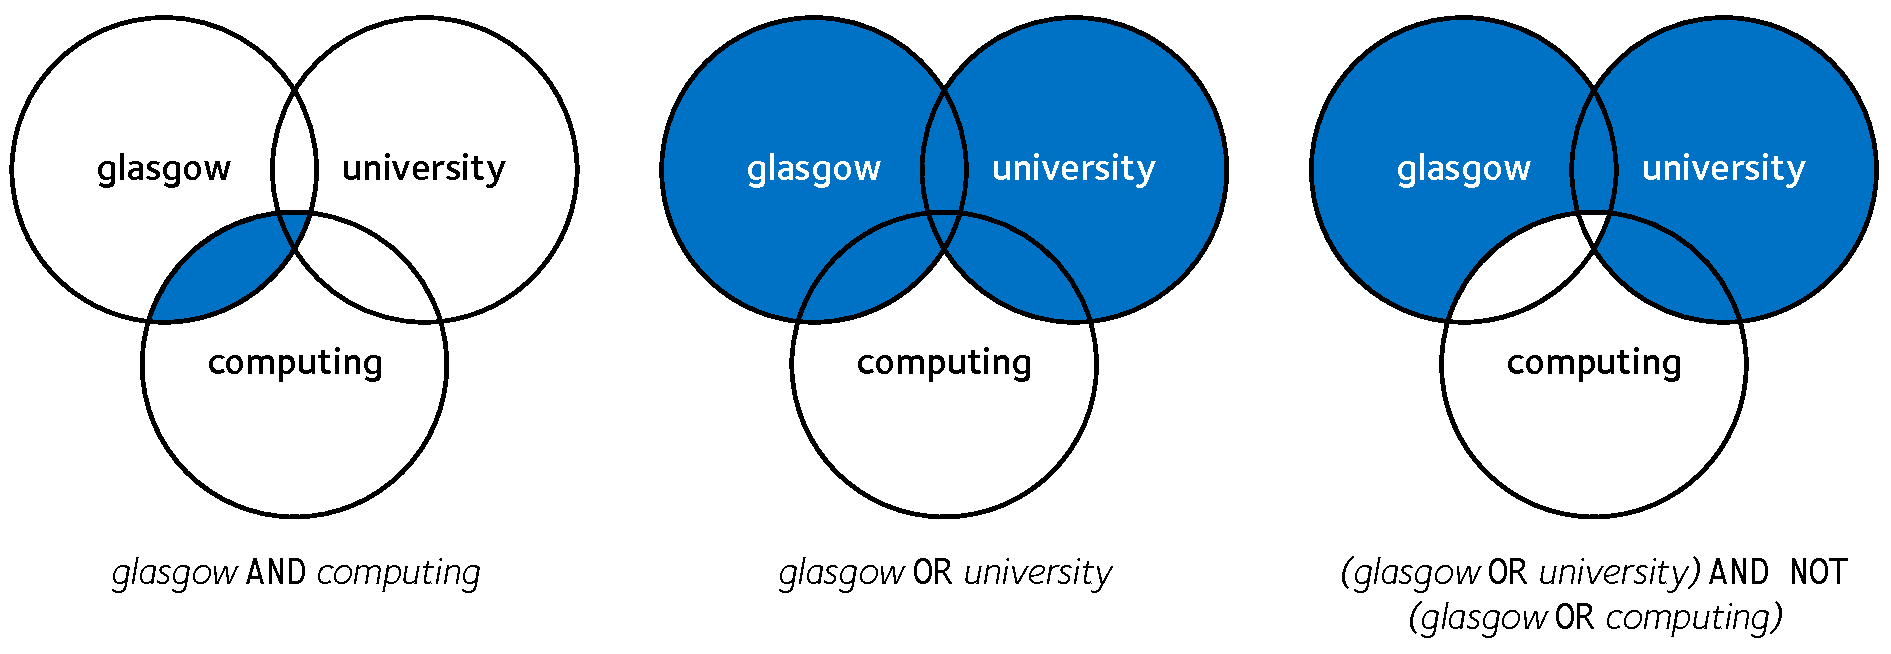
\includegraphics{figures/ch2-boolean.pdf}}
    \caption[Venn diagrams illustrating boolean retrieval]{An example illustration of the boolean retrieval model, using the query terms \texttt{glasgow}, \texttt{university} and \texttt{computing}. Each disc represents the set of documents containing that particular term. In the figure, three Venn diagram examples are provided, demonstrating the key logical operators used (\texttt{AND}, \texttt{OR} and \texttt{NOT}). Areas in blue are returned in the example boolean query provided underneath each Venn diagram.}
    \label{fig:boolean}
\end{figure}

By considering an individual query term as an unambiguous set of documents, logical operations can be applied to retrieve a set of documents. For example, the query term \texttt{glasgow} will yield a set of all documents containing the term \texttt{glasgow}, yet the query \texttt{NOT glasgow} will retrieve the set of documents that \emph{does not} contain any mention of the term \texttt{glasgow}. The results of applying logical operators between different sets can be illustrated through a Venn diagram, where each set of documents is represented as a disc. Figure~\ref{fig:boolean} provides an example of such diagrams.

Despite the relative simplicity of this approach, there are major limitations. First, when considering the query, there is no notion of term importance -- every term has equal weighting. Queries utilising logic rules also appear to be relatively unnatural representations of an information need. Indeed, as the information need become more complex, the boolean query can grow to be disproportionally large and cumbersome to interpret (refer to the right Venn diagram of Figure~\ref{fig:boolean}). This would be especially true when a complex information need is represented as a boolean query. As documents either belong to a set or they don't, a document is either useful (\texttt{TRUE}) or not (\texttt{FALSE}). As such, one cannot estimate a degree to how relevant a document would be to the searcher's query, and thus results are provided to the searcher unranked.

Returning an unranked set of documents would appear as an alien concept to users of~\gls{acr:ir} systems today -- one would assume that the document presented first would be the document considered most likely to be useful as per the underlying retrieval model. This would make it difficult for a searcher to obtain some notion of how many results he or she should examine before stopping, as all terms and documents are considered equal. Despite not being required in contemporary~\gls{acr:ir} systems, many do still provide support for crafting a boolean query for when returning a good set of results is difficult. This may for example be useful when there is ambiguity in the searcher's information need, and clarification is required to eliminate a set of unhelpful documents. Boolean queries also find traction in patent searching, where \emph{recall} rather than \emph{precision} is preferred (refer to Section~\ref{sec:ir_background:evaluation}).

\subsubsection{Vector Space Model}
With major weaknesses present in the boolean retrieval model, work then progressed to develop more advanced approaches that mitigated the issues raised above.~\cite{luhn1957ranking_query} suggested that a searcher, when wishing to search for documents addressing their information need, should prepare a document that is similar to the documents that were sought after. By comparing documents against this \emph{representative} document, a system could begin to deduce what other documents would be useful, and by what margin.

\begin{wrapfigure}{r}{0.45\textwidth}
    \begin{center}
    \vspace*{-8mm}
    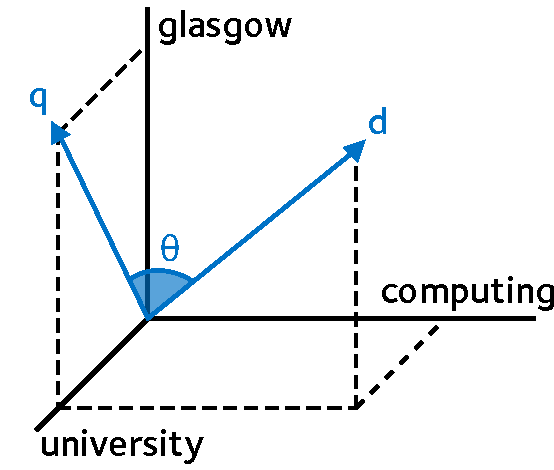
\includegraphics[width=1\textwidth]{figures/ch2-vector.pdf}
    \end{center}
    \vspace*{-2mm}
    \caption[Vector Space Model (Cosine similarity)]{An illustration of the Vector Space Model in Euclidean space, with each term representing a dimension. Here, the cosine similarity between a query \emph{q} and document \emph{d} are shown.}
    \label{fig:vector_space}
\end{wrapfigure}

The Vector Space Model proposed by~\cite{salton1975vsm} incorporates the principles as outlined by~\cite{luhn1957ranking_query}. These basic principles are operationalised by representing queries and documents within Euclidean geometry, where both are represented as vectors in multi-dimensional space. The notion of how close documents appear to each other denotes the usefulness of a document. The Vector Space Model is popular, as it provides an intuitive means for addressing the overarching problem of an~\gls{acr:ir} system, and can incorporate methods such as term weighting which have been shown to improve retrieval effectiveness~\citep{croft2010search}. Indeed, by providing estimates on the degree of relevance, results are returned in a ranked order. This subsequently allows a searcher to decide how many results to examine before stopping.

Consider query $Q$, with each of its terms placed within a term vector in $t$-dimensional space. As such, $Q = (q_1, q_2, q_3,\dotsc, q_{it})$. Consider also a document, $D_i$, with terms from the document again represented in $t$-dimensional space, yielding $D_i = (d_{i1}, d_{i2}, d_{i3},\dotsc, d_{it})$. Essentially, $d_{ij}$ is the \emph{term frequency (TF)} of term $j$ appearing in document $i$. With each term represented as a separate dimension in the Vector Space Model, a weighting scheme can be applied to emphasise more discriminative terms, for example. This addresses the assumption in the boolean model that all terms are of equal weighting. This means that stopword terms, for example (refer to Section~\ref{sec:ir_background:basics:indexing:stopwords}) can be given a lower weighting than terms which are less frequently occurring, and thus more discriminative in allowing one to find particular documents. Other approaches have been trialled, such as \emph{Inverse Document Frequency (IDF)}

Then explain that other approaches include Cosine Similarity, as documents and queries are represented as a series of term vectors. The larger the degree between two vectors, the less relevant two vectors are. So there is a cutoff point there, that determines when someone would stop -- how tolerant is someone before they give up and become frustrated with the results?

\subsubsection{Probabilistic Models}

\subsubsection{Language Models}

% - retrieval models
%     - these models have some notion of how much someone should retrieve/stop.
%     - boolean, look at whole set of documents
%     - other models, there's a cutoff... e.g. cosine similarity, angle gets too large, so you stop.
%     - probabilistic ranking principle
%
%         \begin{quote}
%             ``If a reference retrieval system's response to each request is a ranking of the documents in the collections in order of decreasing probability of usefulness to the user who submitted the request, where the probabilities are estimated as accurately as possible on the basis of whatever data has been made available to the system for this purpose, then the overall effectiveness of the system to its users will be the best that is obtainable on the basis of that data.''
%             \attrib{W.S. Cooper, in private correspondence to~\cite{robertson1977prp}.}
%         \end{quote}
%
%
%         - decreasing probability of relevance
%         - get odds of rel over non-rels, so there is some idea of a cut-off.
%         - why would you look at a document that is less relevant?
%         - nobody uses it, just make this observation.

\subsection{Evaluating Systems}\label{sec:ir_background:evaluation}
- evaluation
    - effects of pooling in judgements?
    - system orientated (cranfield)
        - precision
        - recall
    - user orientated

\subsubsection{Precision}

\subsubsection{Recall}

\subsubsection{Mean Average Precision}

\subsubsection{F-Measure}


\section{User Models}


\begin{figure}[t!]
    \centering
    \resizebox{1\hsize}{!}{
    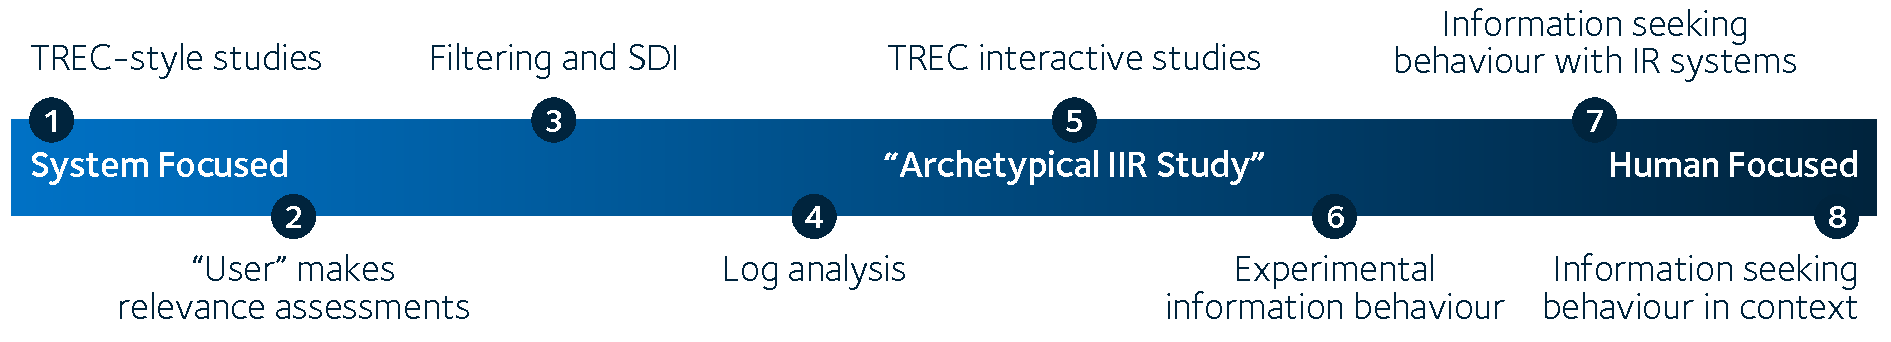
\includegraphics{figures/ch2-spectrum.pdf}}
    \caption[The spectrum of conceptualising IIR research~\citep{kelly2009iir}]{The spectrum of conceptualising IIR research. Methods on the left consider a more system-focused approach, with those on the right considering a more user-focused approach. The fifth step within the spectrum considering TREC interactive studies is considered to be an \emph{"archetypical~\gls{acr:iir} study"}. Figure adapted, with permission, from~\cite{kelly2009iir}.}
    \label{fig:inverted}
\end{figure}

    - diane kelly's spectrum of system to user orientated
        - TREC/Cranfield is a very basic approach to simulation
            a model of how user performs
        - user orientated approach looks at how users interact with the system
        - models of how users search... to show how we develop models.
        
        - at the end of chapter

Look at Kelly (2009) -- Methods for Evaluating Interactive Information Retrieval Systems with Users

these measures/evaluations are thining about the way people go and search
of relevance to this thesis are stopping strats
diff. measures encoe different stopping models. different ways of evaluating this.
in the next chapter, provide an overview of the different types of models of search, and how searching has been conceptualised with respect to stopping strategies.

\subsection{Towards User-Orientated Measures}

Stephen Robertson has good points in his paper on IR evaluation history:~\cite{robertson2008history_ir_evaluation}

Cranfield isn't very good. Furthermore, this model uses only binary and topical-oriented relevance. The conclusion is that the batch-driven mode of the Cranfield model is not suitable for the evaluation of IIR systems, which, if carried out as realistically as possible, requires human interaction, potentially dynamic information need interpretations, and the assignment of multidimensional and dynamic relevance. (From Borlund 2003)

\subsubsection{Relative Relevance}
~\cite{borlund1997iir_evaluation}

\subsubsection{Ranked Half-Life}
~\cite{borlund1997iir_evaluation}

\subsubsection{Cumulative Gain}

\subsubsection{Rank-Biased Precision}

\subsubsection{INST}


\subsection{TREC Ad-Hoc}\label{sec:ir_background:user:trec}
\todo{does this bit need to be moved to the next chapter?}
- searcher acquires an information need, sits down, and conducts a search against an existing collection of documents over a set period of time. Known as ad-hoc retrieval, or retrospective searching in older literature.

- this is lifted from Robertson (2008), rephrasing required, and probably needs to be moved to the user model part.

- The user model invoked here is what has now become the most obvious one for search: user has an
information need, sits down in front of a system and conducts a search against an existing collection of
documents, over a limited time period. This is known in TREC jargon as an ‘ad-hoc’ search – an earlier more-orless
equivalent term was ‘retrospective searching’. System produces a ranked list of items, which the user consults
in rank order. Users may judge documents good or bad, but in principle there may be any number of good
documents in the collection. (The one significant change in this model from the Cranfield view is that there is now
an assumption that each system will rank its results list.) It is often asserted that there is also an assumption that
requests are topical or subject-based (documents about X); indeed the TREC jargon, which is to call requests
‘topics’, encourages that view18. However, although most of the requests used in TREC (all of those in early
TRECs) are indeed topical, there is no necessary requirement of the model that this should be so, or that they
should be purely topical. In some sense the nature of the requests is determined by the relevance judgements; if
the judgements depend on other criteria than pure topicality, then that is the nature of the task.
However, it is fundamental to the model that the judge or assessor should indeed be able to make a judgement
on each document, actually a binary one for most of the TREC ad-hoc tasks, and should be able to make the
judgement irrespective of the order of presentation of the documents. This last precludes, for example, embedding
a criterion of novelty in the usual ad-hoc task relevance judgements (although one track did investigate novelty by
making judgements of novelty separated from the relevance judgements). A typical TREC ‘topic’ has a short title (which might be used directly as a query), and additional information about the
supposed information need under the headings ‘description’ and ‘narrative’. The narrative contains explicit rules for
judging the relevance of documents. An example title and description are: Hydroponics—Document will discuss the
science of growing plants in water or some substance other than soil. 

\section{Chapter Summary}



Basic concepts -- given a query, tries to satisfy that query.
Follows a system-orientated methodology

From Leif:
- indexing
    tokenizers, etc
- retrieval models
    - these models have some notion of how much someone should retrieve/stop.
    - boolean, look at whole set of documents
    - other models, there's a cutoff... e.g. cosine similarity, angle gets too large, so you stop.
    - probabilistic ranking principle
    
        \begin{quote}
            ``If a reference retrieval system's response to each request is a ranking of the documents in the collections in order of decreasing probability of usefulness to the user who submitted the request, where the probabilities are estimated as accurately as possible on the basis of whatever data has been made available to the system for this purpose, then the overall effectiveness of the system to its users will be the best that is obtainable on the basis of that data.''
            \attrib{W.S. Cooper, in private correspondence to~\cite{robertson1977prp}.}
        \end{quote}
    
    
        - decreasing probbaility of relevance
        - get odds of rel over non-rels, so there is some idea of a cut-off.
        - why would you look at a document that is less relevant?
        - nobody uses it, just make this observation.
- evaluation
    - effects of pooling in judgements?
    - system orientated (cranfield)
        - precision
        - recall
    - user orientated
    
    - diane kelly's spectrum of system to user orientated
        - TREC/Cranfield is a very basic approach to simulation
            a model of how user performs
        - user orientated approach looks at how users interact with the system
        - models of how users search... to show how we develop models.
        
        - at the end of chapter

% \subsection{Methodologies}
%
% \subsubsection{System-Orientated}
%
% \subsubsection{User-Orientated}
%
% \subsection{Retrieval Models}
%
% \subsubsection{Boolean Model}
%
% \subsubsection{Vector Space Model}
%
% \subsubsection{Probabilistic Models}
%
% \subsubsection{Language Models}
%
% \subsection{Search Tasks}
%
% \section{Evaluating Retrieval Effectiveness}\label{sec:ir_background:evaluation}
% Basic measures and models.
%
% \subsection{Precision}
%
% \subsection{Recall}
%
% \subsection{Mean Average Precision}
%
% \subsection{F-Measure}
%
% \subsection{Towards User-Orientated Measures}
%
% \subsection{User Models}
% these measures/evaluations are thining about the way people go and search
% of relevance to this thesis are stopping strats
% diff. measures encoe different stopping models. different ways of evaluating this.
% in the next chapter, provide an overview of the different types of models of search, and how searching has been conceptualised with respect to stopping strategies.